\section{Domain Driven Design}
	
		\subsection{Model the Core Domain and the corresponding Bounded Context of your
			application. Please explain, why your solution is the Core Domain.}
			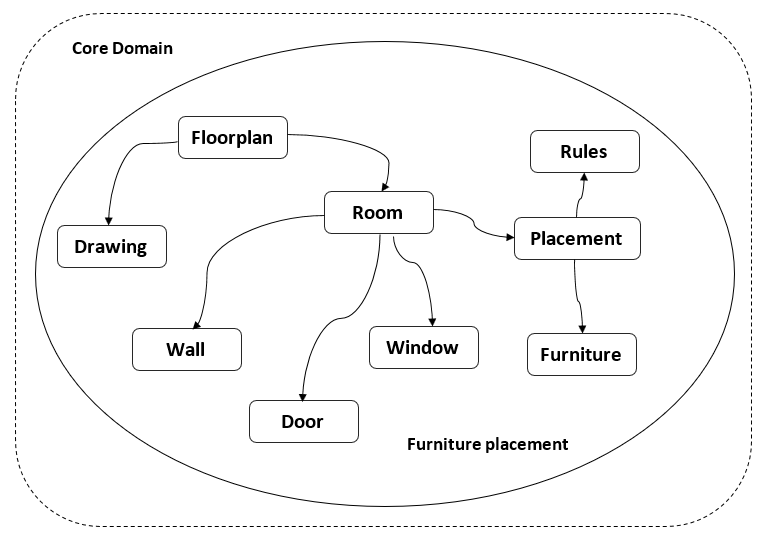
\includegraphics[keepaspectratio,width=0.8\textwidth,angle=0]{images/ddd1.PNG}
			\newline
			Core domain is the most important subdomain and is a foundational concept behind the business.
            In our example, the most important part of the task is the placement of furniture according to the floorplan. The floorplan has information about rooms. Additionally, some rules must be considered in the placement.
            
		\subsection{Model necessary Subdomains and their corresponding Bounded Context and
			classify them as Supporting or Generic Subdomains.}
			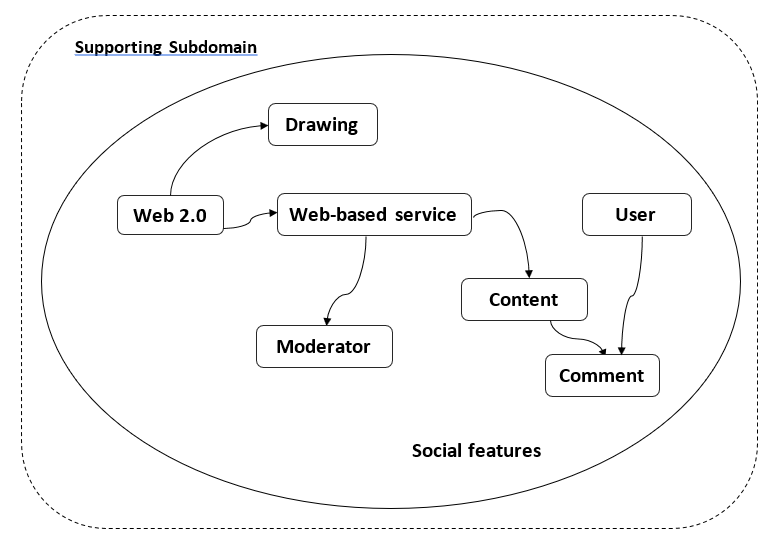
\includegraphics[keepaspectratio,width=0.8\textwidth,angle=0]{images/ddd2.PNG}
			\newline
		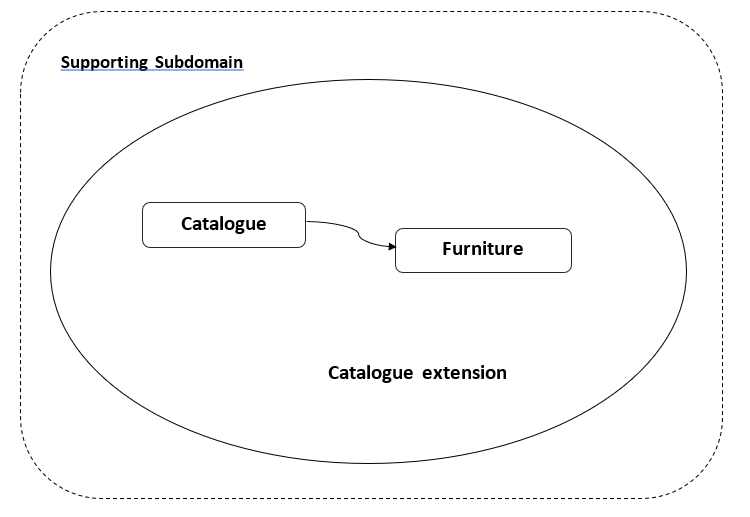
\includegraphics[keepaspectratio,width=0.8\textwidth,angle=0]{images/ddd3.PNG}
		
		\subsection{Create a Context Map for your Bounded Contexts and explain the relationships
			between the contexts.}
			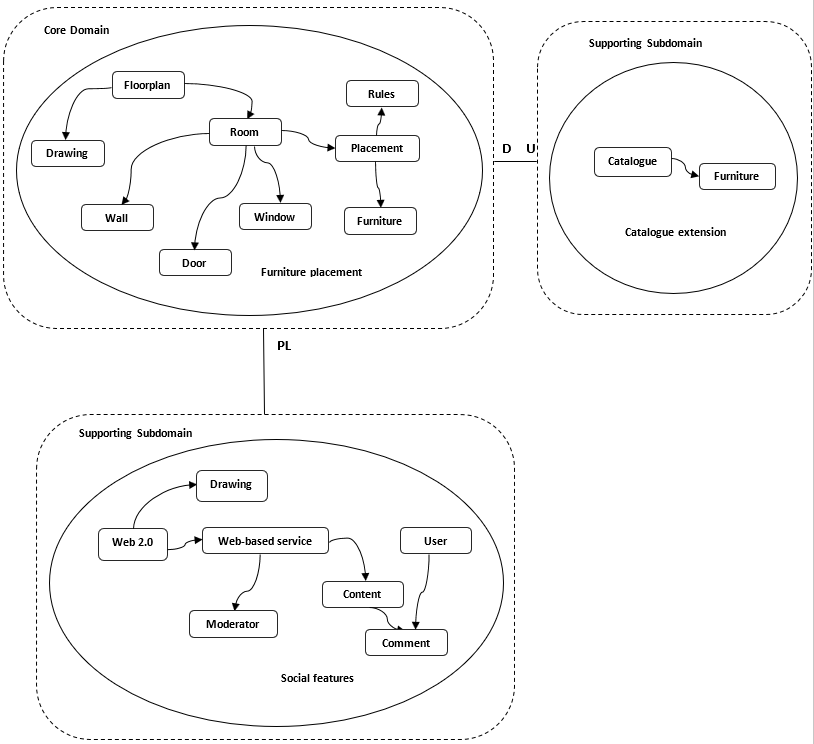
\includegraphics[keepaspectratio,width=0.8\textwidth,angle=0]{images/ddd4.PNG}
			\newline
			Here we have one Core domain and two supporting subdomains, including Catalog extension and Social features.
            Catalog extension is upstream for the Core domain because the Core domain uses furniture created in Catalog extension.
            Further, the core domain publishes results for Social features. The publishing language can be JSON/XML-Schema. Also, we can use REST as a technique.